\documentclass{article}
\usepackage[utf8]{inputenc}
\usepackage{amsmath}
\usepackage{siunitx}
\usepackage{graphicx}
\usepackage{caption}
\usepackage{subcaption}
\usepackage{float}
\usepackage{enumitem}
\usepackage{amssymb}
\usepackage{pgfplots}
\usepackage[superscript]{cite}
\usepackage{todonotes}
\usepackage{tikz}
\usepackage{tabularx}
\usepackage{float}

\pgfplotsset{compat=1.16}
%\pgfplotsset{
%    dirac/.style={
%        mark=triangle*,
%        mark options={scale=1},
%        ycomb,
%        scatter,
%        visualization depends on={y/abs(y)-1 \as \sign},
%        scatter/@pre marker code/.code={\scope[rotate=90*\sign,yshift=-2pt]}
%    }
%}


\title{Implementation and Review of \\ \textit{Data Cache Prefetching Using a Global History Buffer\cite{GHB}} \\ NUS CS5222, Project 3}
\author{Luca Krueger}
\date{\today}

\begin{document}
\maketitle

\section{Introduction}
This project covers an implementation based review of the \textit{GHB PC/DC prefetcher} introduced by \textit{Kyle J. Nesbit} and \textit{James E. Smith} in the paper \textit{Data Cache Prefetching Using a Global History Buffer\cite{GHB}}. \\
The review focuses on the performance of the proposed algorithm, but does not discuss feasibility from a hardware point of view.
For better comparison, we use the infrastructure from the \textit{2nd Data Prefetching Championship (DPC2)}. The implementation is compared against the default \textit{No prefetching} skeleton and other example prefetchers which were provided. \\
The IPC of several benchmarks will be taken as performance reference value of the prefetchers. The idea is, that cache misses cause a significant delay, which will affect the accumulated IPC value. 
Of course, IPC does not only depend on caching performance and memory access delays. Therefore, the actual number of cache misses in relation to the number of memory accesses might give more accurate view on the prefetcher's performance, but in the end it is only the overall IPC improvement which matters. 


\section{The Prefetching Algorithm}
The \textit{Global History Buffer Programm Counter/Delta Correlation (GHB PC/DC)} prefetcher contains of two linked tables to detect recurring memory access patterns and uses this knowledge to prefetch data chunks from the memory which might be accessed later during code execution. \\
The \textit{Index Table's (IT)} entries are dedicated to a single instruction pointer value each, such that a unique mapping of instruction pointers is possible within the range of table size \texttt{IT\_SIZE}. \\
A field in the IT points to an entry in the \textit{Global History Table (GHB)}, when initialized successfully after the first occurrance of a cache miss by the corresponding instruction pointer. \\
The GHB is a circular buffer of all past \texttt{GHB\_SIZE} cache misses. Entries in the GHB are linked by the instruction pointer of the calling instruction and store the accessed memory address.
In other words, an entry in the IT corresponds to a particular instruction pointer and refers to the most recent memory request in the GHB called by this instruction pointer. \\
The GHB keeps track of all most recent cache misses. Therefore, a new occurrance of a cache miss is inserted at the current position of the GHB and referenced in the IT at the position of the calling instruction pointer. If this position in the IT previously pointed to another entry in the GHB and the full instruction pointer values still match, the new entry in the GHB will point to the previous occurrance.
Over the time, most of the entries in the GHB are interconnected through linked lists, where elements within a linked list share the same instruction pointer value. The stored miss addresses are uses to create so called delta access patterns, namely the difference between two adjacent cache miss addresses. On each occurrance of a new cache miss, the address deltas to the two preceding cache misses define an access pattern. If such a pattern occured previously and is found in the linked list, the data will be prefetched into the L2 cache accordingly.


\section{Implementation and Performance}
The implementation follows the description of the \textit{GHB PC/DC} prefetcher as proposed in the paper, but also introduces a few changes.
Since the GHB is a circular buffer, problems arise when valid entries in the table are overwritten by a new entry. 
The problem is solved here, by storing the full instruction pointer value in the GHB and comparing it every time when referencing to any entry. 
The author's also identify this as major problem of the algorithm and observed that storing the instruction pointer value with only 4 bit more accuracy than in the IT reduces errors to a negligible amount.
This method also prevents aliasing caused by the truncated indexing in the IT.


\begin{figure}[H]
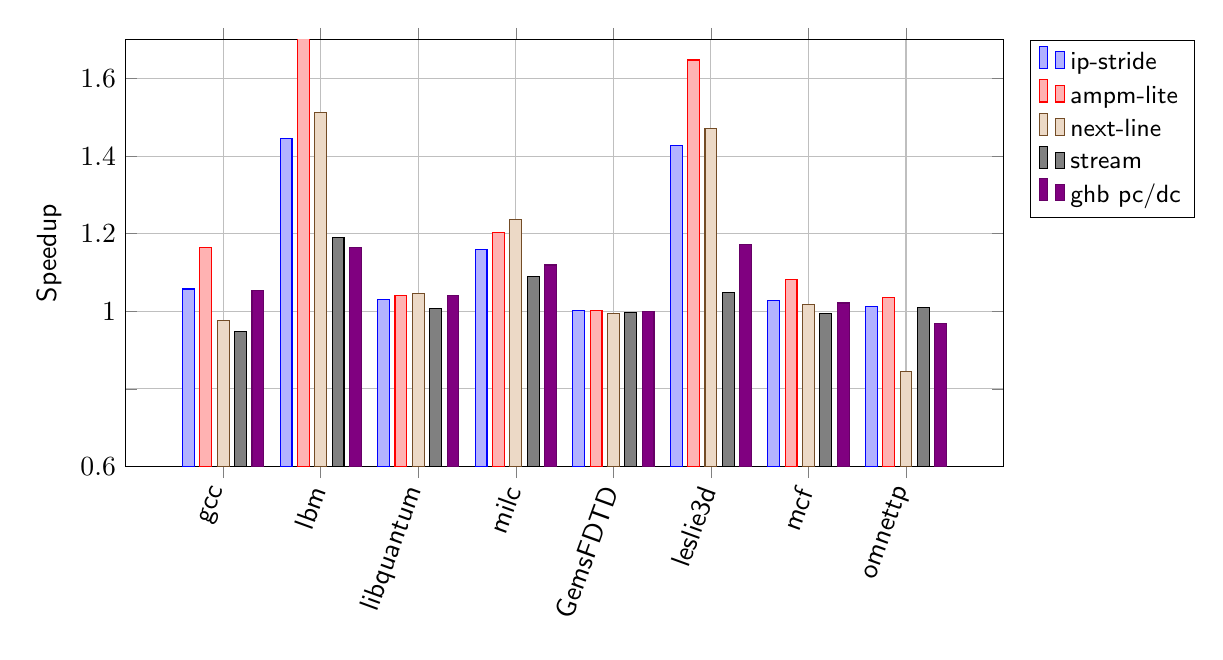
\begin{tikzpicture}
	\begin{axis}[
		width=1.05\textwidth,
		height=7cm,
		xmin=0, xmax=9,
		ymin=0.6, ymax=1.7,
		ylabel=\textsf{Speedup},
		ytick={0.6,0.8,1,1.2,1.4,1.6},
		yticklabels={0.6,,1,1.2,1.4,1.6},
		ybar,
		bar width=0.15cm,
		xtick={1,2,3,4,5,6,7,8}, 
		xticklabels={\textsf{gcc}, \textsf{lbm}, \textsf{libquantum}, \textsf{milc}, \textsf{GemsFDTD}, \textsf{leslie3d}, \textsf{mcf}, \textsf{omnettp}},
		ytick distance ={10},
		xmajorgrids=true,
		ymajorgrids=true,
		x tick label style={rotate=70,anchor=east},
		legend pos=outer north east,
		legend cell align=left,
		legend style={font=\small\sf}
	]
		% ip-stride
		\addplot
			coordinates {(1,1.0574058881882682) (2,1.4461944168138547) (3,1.030055362550216) (4,1.1596194524733754) (5,1.0011582019712655) (6,1.4283652396858797) (7,1.0266428911631795) (8,1.013054072685449)};

		% ampm-lite
		\addplot
			coordinates {(1,1.1641717782987617) (2,1.924160649921899) (3,1.0400129345518665) (4,1.2029909779067847) (5,1.001837157963945) (6,1.6478760732298243) (7,1.0824262630252197) (8,1.0353873815345072)};

		% next-line
		\addplot
			coordinates {(1,0.9756804162990983) (2,1.512943407929622) (3,1.0461498584727509) (4,1.2362582892903695) (5,0.994292299408272) (6,1.4701322639351135) (7,1.0182324036104689) (8,0.845492209210072)};

		% stream
		\addplot
			coordinates { (1,0.9475301120039542) (2,1.1905902398251142) (3,1.007593013944349) (4,1.0893866486075217) (5,0.9979425224129498) (6,1.048952170413519) (7,0.994345573458174) (8,1.0104959981896844)};

		% ghb pc/dc ghb:512 it:256 semi-accurate
		\addplot
			coordinates {(1,1.0537845528594818) (2,1.16365860946063) (3,1.040118393078871) (4,1.119378020198229) (5,1.0004470253222428) (6,1.1713128040542942) (7,1.0213631030517059) (8,0.9679499316341248)};

		\legend{ip-stride, ampm-lite, next-line, stream, ghb pc/dc}
	\end{axis}
\end{tikzpicture}
\caption{Speedup: GHB PC/DC (GHB size 512, IT size 256) speedup compared to other prefetchers}
\label{speedup-general}
\end{figure}

The implementation's speedup over \textit{No prefetching} is compared to other example prefetchers (Figure \ref{speedup-general}) from the DPC2 infrastructure. 
The GHB prefetcher shows a constant performance in the average field of all tested prefetcher. 
Where other prefetchers show outstanding performance for some benchmarks, such as \texttt{ampm-lite} for the \textit{lbm} and \textit{leslie3d} benchmark, this prefetcher does not seem to have strong specialization for any type of application.
The \texttt{next-line} prefetcher is expected to perform the best for memory accesses with strong locality, but both causes large cache overhead when it comes to more complex access patterns of small data chunks without strong locality.

\paragraph{Variations} The GHB provides usefull additional information that can be used to prefetch a specific pattern which has already been seen in the past and therefore still resides in the GHB. 
\textit{Delta1} and \textit{Delta2} are the distances from the current miss address to the two preceeding misses caused by the same instruction pointer. 
The \textit{primitive} implementation would be to prefetch a data of size \textit{Delta1} before or after the current miss address depending on whether \textit{Delta1} is positive or negative. \\\\
One might argue that this strategy throws away information such as \textit{Delta2} which could also be used for prefetching. 
Benchmark tests showed that the \textit{primitive} implementation shows surprisingly good results and a more complex strategy which takes all available information into account does not perform much better.
The benchmark results comparing the different variants are shown in Figure \ref{speedup-variants}. 
The \textit{accurate} implementation uses both \textit{Delta1} and \textit{Delta2} and prefetches a data chunk with covers the whole range accordingly. 
The so called \textit{semi-accurate} implementation takes the larger of the two deltas as upper limit when larger than zero and the smaller of the two as lower limit when smaller than zero respectively. 

\begin{figure}[H]
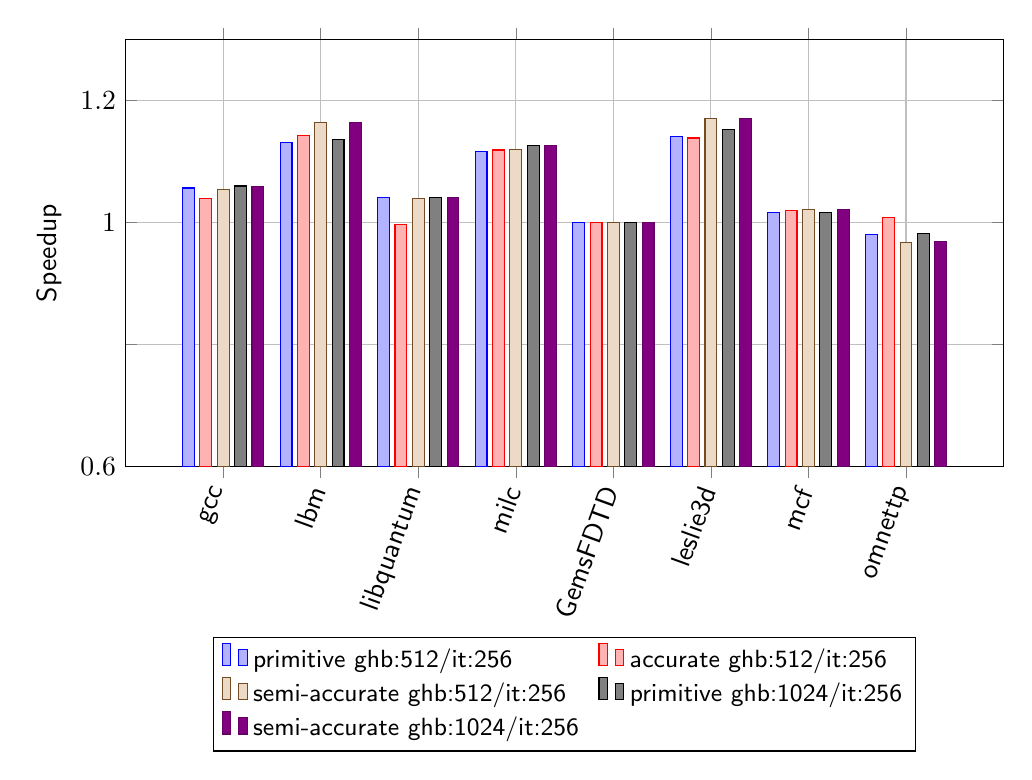
\begin{tikzpicture}
	\begin{axis}[
		width=1.05\textwidth,
		height=7cm,
		xmin=0, xmax=9,
		ymin=0.6, ymax=1.3,
		ylabel=\textsf{Speedup},
		ytick={0.6,0.8,1,1.2},
		yticklabels={0.6,,1,1.2},
		ybar,
		bar width=0.15cm,
		xtick={1,2,3,4,5,6,7,8}, 
		xticklabels={\textsf{gcc}, \textsf{lbm}, \textsf{libquantum}, \textsf{milc}, \textsf{GemsFDTD}, \textsf{leslie3d}, \textsf{mcf}, \textsf{omnettp}},
		ytick distance ={10},
		xmajorgrids=true,
		ymajorgrids=true,
		x tick label style={rotate=70,anchor=east},
		legend cell align=left,
		legend columns=2,
		legend style={at={(0.5,-0.4)},/tikz/column 2/.style={column sep=5pt}, anchor=north,font=\small\sf}
	]
		% ghb pc/dc primitive ghb:512/it:256
		\addplot
			coordinates {(1,1.0567571371198885) (2,1.1320938650005106) (3,1.0415716242868447) (4,1.1166028545144122) (5,1.0003924533997872) (6,1.1412831763644318) (7,1.0163446905893148) (8,0.9800915468572)};

		% ghb pc/dc accurate ghb:512/it:256
		\addplot
			coordinates {(1,1.0388873061040953)(2,1.1431235131485886) (3,0.9975925597103322) (4,1.1191730189845404) (5,1.0002267056991374) (6,1.1387680199588521) (7,1.0197716157661791) (8,1.0076354440451432)};

		% ghb pc/dc semi-accurate ghb:512/it:256
		\addplot
			coordinates {(1,1.0537845528594818) (2,1.16365860946063) (3,1.040118393078871) (4,1.119378020198229) (5,1.0004470253222428) (6,1.1713128040542942) (7,1.0213631030517059) (8,0.9679499316341248)};

%		% ghb pc/dc semi-accurate ghb:512/it:256 check bounds
%		\addplot
%			coordinates {(1,1.0435590003054964) (2,1.162998627085374) (3,1.0415697184098507) (4,1.1217758204638129) (5,1.0004470253222428) (6,1.171760416634948) (7,1.0172943554476492) (8,0.991502283652914)};

		% ghb pc/dc primitive ghb:1024/it:256
		\addplot
			coordinates {(1,1.0600695433684941) (2,1.1368347699138808) (3,1.0415827419026433) (4,1.125954377540842) (5,1.0003924533997872) (6,1.152939373362687) (7,1.0169081003217824) (8,0.9826464277518464)};

		% ghb pc/dc semi-accurate ghb:1024/it:256
		\addplot
			coordinates {(1,1.058936803407831) (2,1.1648991493980734) (3,1.0411478843018311) (4,1.1261043038015996) (5,1.0004470253222428) (6,1.170105975577202) (7,1.0213021154002533) (8,0.9685699464798077)};

		\legend{primitive ghb:512/it:256, accurate ghb:512/it:256, semi-accurate ghb:512/it:256, primitive ghb:1024/it:256, semi-accurate ghb:1024/it:256}
	\end{axis}
\end{tikzpicture}
\caption{Speedup: Variants of GHB PC/DC}
\label{speedup-variants}
\end{figure}

Surprisingly, the \textit{semi-accurate} implementation shows the best overall performance of all variants. The fact that the \textit{semi-accurate} implementation shows a better performance than the \textit{accurate} implementation might indicate that the actual memory access pattern does not strictly have to be the same as the past delta pair pattern. In other words, the delta pair can be used to predict a new prefetch candidate, but does not necessarly have to be the candidate. \\
Tests showed that the Delta can become very large when the applications accesses different regions in the memory. 
A large Delta of course can be a good indicator to predict the next memory access, but prefetching the whole stride covered by this Delta is obviously not possible and not required.  \\
Prefetching into the $L2$ cache is limited by first the cache size and second it's occupancy. 
Hence, any prefetcher needs a mechanism to check whether a prefetch is feasible. 
Interestingly enough, a simple mechanism which excludes large Deltas from beeing prefetched causes a significant drop in the IPC speedup for all variants. 
Thankfully, the simulators function for cache prefetches provided by the DPC2 infrastructure denies unrealistic requests without any additional cost. 
According to the heartbeat statistics, using the inbuild mechanism appears to be a great advantage especially in the beginning of program execution.


\section{Conclusion}
Not any of the implementation variants shows as high IPC speedups as promised in the original paper. On the other hand the implemented \textit{GHB PC/DC} prefetcher gives an IPC speedup ranging in the average field of all tested prefetchers. The best performing prefetcher, the \texttt{ampm-lite} prefetcher is counted to the state of the art prefetchers and also uses Delta Correlation prefetching combined with other mechanisms, namely an advancement of the \textit{GHB PC/DC} prefetcher.
The implementation indeed suffers significant issues: 
\begin{itemize}
	\item Recent data in GHB and IT is sparse and old data tends to stale. 
	\item Fast recurring memory accesses following the same pattern congest the GHB with redundant data. 
\end{itemize}
To solve these issues, the algorithm needs to perform additional filtering, to avoid dublicate prefetches until the prefetched data arrives in the cache. 
Linked lists instead of arrays and tables of fixed size would make a better memory usage possible, but come with a large overhead because searching and matching becomes more complicated.


\bibliography{references}
\bibliographystyle{unsrt}
\end{document}
